% ============================================================================
% Chapitre 5 : R\'eseaux R\'ecurrents et LSTM
% ============================================================================
\chapter{R\'eseaux R\'ecurrents et LSTM}
\label{ch:rnn_lstm}

\noindent\textit{Ce chapitre \'etudie les r\'eseaux de neurones r\'ecurrents (RNN), con\c{c}us
pour traiter des donn\'ees s\'equentielles. Nous d\'erivons les \'equations de
propagation, analysons le probl\`eme fondamental de la disparition et de
l'explosion des gradients, puis pr\'esentons les architectures LSTM et GRU qui
r\'esolvent partiellement ce probl\`eme.}\medskip

% ----------------------------------------------------------------------------
\section{Motivation : donn\'ees s\'equentielles}
\label{sec:rnn-motivation}
\index{donn\'ees s\'equentielles}

De nombreux probl\`emes impliquent des donn\'ees ordonn\'ees dans le temps ou
dans l'espace :
\begin{itemize}
  \item \textbf{S\'eries temporelles} : pr\'evision financi\`ere, m\'et\'eorologie,
    signaux physiologiques.
  \item \textbf{Traitement du langage naturel} : traduction, analyse de sentiment,
    g\'en\'eration de texte.
  \item \textbf{Audio} : reconnaissance vocale, synth\`ese musicale.
\end{itemize}

Les r\'eseaux de neurones classiques (MLP, CNN du chapitre~\ref{ch:cnn})
traitent des entr\'ees de taille fixe et ne capturent pas naturellement les
d\'ependances temporelles.

\begin{definition}[S\'equence]
Une s\'equence de longueur $T$ est un ensemble ordonn\'e
$\mathbf{x} = (x_1, x_2, \ldots, x_T)$ o\`u chaque $x_t \in \R^d$ est un
vecteur d'entr\'ee au pas de temps $t$.
\end{definition}

% ----------------------------------------------------------------------------
\section{Architecture RNN}
\label{sec:rnn-arch}
\index{RNN}

\subsection{\'Equations de r\'ecurrence}

Un RNN simple (<<~Vanilla RNN~>>) maintient un \'etat cach\'e
$h_t \in \R^{d_h}$ qui r\'esume l'information des pas de temps pr\'ec\'edents :

\begin{formules}[title=\textbf{RNN -- \'Equations fondamentales}]
\begin{align}
h_t &= \tanh(W_{hh} h_{t-1} + W_{xh} x_t + b_h)
\label{eq:rnn-hidden} \\
y_t &= W_{hy} h_t + b_y
\label{eq:rnn-output}
\end{align}
o\`u :
\begin{itemize}
  \item $W_{xh} \in \R^{d_h \times d}$ : poids entr\'ee $\to$ cach\'e
  \item $W_{hh} \in \R^{d_h \times d_h}$ : poids cach\'e $\to$ cach\'e (r\'ecurrence)
  \item $W_{hy} \in \R^{d_y \times d_h}$ : poids cach\'e $\to$ sortie
  \item $b_h, b_y$ : biais
\end{itemize}
\end{formules}

\begin{remarque}[Partage des param\`etres]
Les matrices $W_{xh}$, $W_{hh}$ et $W_{hy}$ sont \textbf{partag\'ees} \`a
travers tous les pas de temps, ce qui permet de traiter des s\'equences de
longueur variable.
\end{remarque}

\subsection{Graphe de calcul d\'epli\'e}

\begin{center}
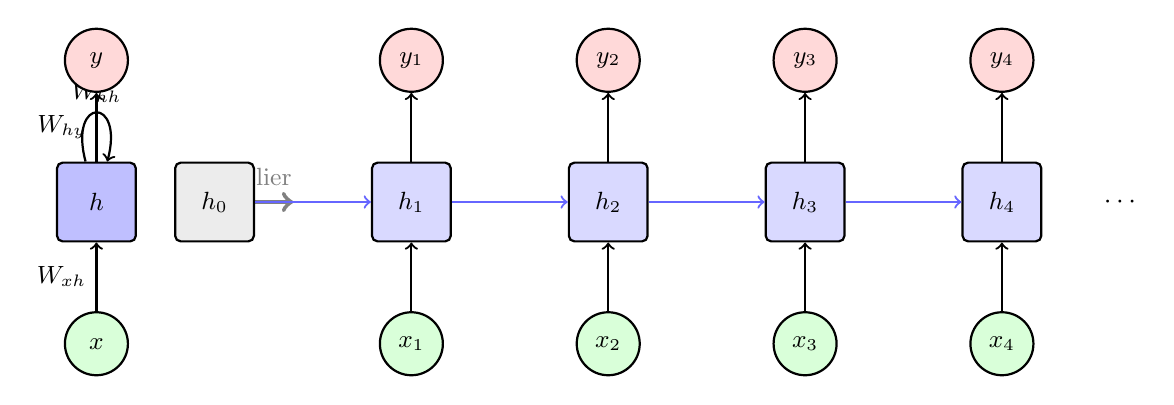
\begin{tikzpicture}[
  rnn/.style={rectangle, draw, thick, fill=blue!15, minimum size=10mm,
              rounded corners=2pt, font=\small},
  input/.style={circle, draw, thick, fill=green!15, minimum size=8mm,
                font=\small},
  output/.style={circle, draw, thick, fill=red!15, minimum size=8mm,
                 font=\small},
  arr/.style={->, thick},
  harr/.style={->, thick, blue!60}
]
  % \'Etat compact
  \node[rnn, fill=blue!25] (compact) at (-3, 0) {$h$};
  \draw[arr, loop above, looseness=8, thick] (compact) to
    node[above, font=\small] {$W_{hh}$} (compact);
  \node[input] (ci) at (-3, -1.8) {$x$};
  \node[output] (co) at (-3, 1.8) {$y$};
  \draw[arr] (ci) -- (compact) node[midway, left, font=\small] {$W_{xh}$};
  \draw[arr] (compact) -- (co) node[midway, left, font=\small] {$W_{hy}$};

  % Fl`eche de d'epliage
  \draw[->, ultra thick, gray] (-1.5, 0) -- (-0.5, 0)
    node[midway, above, font=\small] {d\'eplier};

  % RNN d'epli'e
  \foreach \t in {1,2,3,4} {
    \pgfmathsetmacro{\x}{\t * 2.5 - 1.5}
    \node[rnn] (h\t) at (\x, 0) {$h_{\t}$};
    \node[input] (x\t) at (\x, -1.8) {$x_{\t}$};
    \node[output] (y\t) at (\x, 1.8) {$y_{\t}$};
    \draw[arr] (x\t) -- (h\t);
    \draw[arr] (h\t) -- (y\t);
  }

  % Connexions r'ecurrentes
  \node[rnn, fill=gray!15] (h0) at (-1.5, 0) {$h_0$};
  \draw[harr] (h0) -- (h1);
  \draw[harr] (h1) -- (h2);
  \draw[harr] (h2) -- (h3);
  \draw[harr] (h3) -- (h4);

  % Points de suspension
  \node at (10, 0) {$\cdots$};
\end{tikzpicture}
\end{center}

% ----------------------------------------------------------------------------
\section{R\'etropropagation \`a travers le temps (BPTT)}
\label{sec:bptt}
\index{BPTT}\index{r\'etropropagation!travers le temps}

\subsection{D\'erivation compl\`ete}

La perte totale sur une s\'equence de longueur $T$ est :
\begin{equation}
\mathcal{L} = \sum_{t=1}^T \mathcal{L}_t(y_t, \hat{y}_t)
\end{equation}

Le gradient par rapport \`a $W_{hh}$ n\'ecessite de sommer les contributions
de tous les pas de temps :

\begin{theoreme}[Gradient BPTT par rapport \`a $W_{hh}$]
\begin{align}
\frac{\partial \mathcal{L}}{\partial W_{hh}}
&= \sum_{t=1}^T \frac{\partial \mathcal{L}_t}{\partial W_{hh}} \nonumber \\
&= \sum_{t=1}^T \frac{\partial \mathcal{L}_t}{\partial y_t}
   \frac{\partial y_t}{\partial h_t}
   \sum_{k=1}^{t} \left(\prod_{j=k+1}^{t}
   \frac{\partial h_j}{\partial h_{j-1}}\right)
   \frac{\partial h_k}{\partial W_{hh}}
\label{eq:bptt-whh}
\end{align}
\end{theoreme}

\textbf{D\'emonstration.}
Par la r\`egle de la cha\^ine, $h_t$ d\'epend de $W_{hh}$ \`a la fois
directement (au temps $t$) et indirectement (via $h_{t-1}, h_{t-2}, \ldots$).
On a :
\begin{align}
\frac{\partial \mathcal{L}_t}{\partial W_{hh}}
&= \frac{\partial \mathcal{L}_t}{\partial h_t}
   \cdot \frac{\partial^+ h_t}{\partial W_{hh}}
   + \frac{\partial \mathcal{L}_t}{\partial h_t}
   \cdot \frac{\partial h_t}{\partial h_{t-1}}
   \cdot \frac{\partial \mathcal{L}_{t-1}}{\partial W_{hh}}
\end{align}

En d\'eroulant la r\'ecurrence, on obtient une somme de produits de Jacobiennes :
\begin{equation}
\frac{\partial h_t}{\partial h_k}
= \prod_{j=k+1}^{t} \frac{\partial h_j}{\partial h_{j-1}}
= \prod_{j=k+1}^{t} W_{hh}^\top \cdot \text{diag}(\tanh'(z_j))
\label{eq:jacobian-product}
\end{equation}
o\`u $z_j = W_{hh} h_{j-1} + W_{xh} x_j + b_h$.

% ----------------------------------------------------------------------------
\section{Disparition et explosion des gradients}
\label{sec:vanishing-exploding}
\index{disparition des gradients}\index{explosion des gradients}

\subsection{Analyse par les valeurs singuli\`eres}

\begin{theoreme}[Condition de disparition/explosion]
Soit $\sigma_{\max}$ la plus grande valeur singuli\`ere de $W_{hh}$ et
$\gamma = \max |\tanh'(z)| \leq 1$. Alors :
\begin{equation}
\left\|\frac{\partial h_t}{\partial h_k}\right\|
= \left\|\prod_{j=k+1}^{t} W_{hh}^\top \text{diag}(\tanh'(z_j))\right\|
\leq (\sigma_{\max} \cdot \gamma)^{t-k}
\label{eq:gradient-bound}
\end{equation}

\begin{itemize}
  \item Si $\sigma_{\max} \cdot \gamma < 1$ : le gradient
    \textbf{d\'ecro\^it exponentiellement} avec $(t-k)$ $\to$
    \emph{disparition des gradients}.
  \item Si $\sigma_{\max} \cdot \gamma > 1$ : le gradient
    \textbf{cro\^it exponentiellement} $\to$ \emph{explosion des gradients}.
\end{itemize}
\end{theoreme}

\begin{attention}[title=\textbf{Cons\'equence pratique}]
Pour $t - k = 100$ et $\sigma_{\max} \gamma = 0.9$ :
$\|\partial h_t / \partial h_k\| \leq 0.9^{100} \approx 2.66 \times 10^{-5}$.
Le RNN ne peut pas apprendre de d\'ependances au-del\`a de 10--20 pas de temps.
\end{attention}

\subsection{Gradient Clipping}
\index{gradient clipping}

Pour combattre l'explosion des gradients :
\begin{formules}[title=\textbf{Gradient Clipping par norme}]
\begin{equation}
\hat{g} = \begin{cases}
g & \text{si } \|g\| \leq \tau \\[4pt]
\dfrac{\tau}{\|g\|} \cdot g & \text{si } \|g\| > \tau
\end{cases}
\label{eq:grad-clip}
\end{equation}
\end{formules}

% ----------------------------------------------------------------------------
\section{Long Short-Term Memory (LSTM)}
\label{sec:lstm}
\index{LSTM}

Le LSTM \cite{hochreiter1997long} r\'esout le probl\`eme de la disparition
des gradients en introduisant une \textbf{cellule m\'emoire} $c_t$ et des
\textbf{portes} (gates) qui contr\^olent le flux d'information.

\subsection{Les quatre portes}

\begin{formules}[title=\textbf{\'Equations du LSTM}]
\begin{align}
\text{Porte d'oubli :} \quad
f_t &= \sigmoid(W_f [h_{t-1}, x_t] + b_f)
\label{eq:lstm-forget} \\
\text{Porte d'entr\'ee :} \quad
i_t &= \sigmoid(W_i [h_{t-1}, x_t] + b_i)
\label{eq:lstm-input} \\
\text{Candidat cellule :} \quad
\tilde{c}_t &= \tanh(W_c [h_{t-1}, x_t] + b_c)
\label{eq:lstm-candidate} \\
\text{Mise \`a jour cellule :} \quad
c_t &= f_t \odot c_{t-1} + i_t \odot \tilde{c}_t
\label{eq:lstm-cell} \\
\text{Porte de sortie :} \quad
o_t &= \sigmoid(W_o [h_{t-1}, x_t] + b_o)
\label{eq:lstm-output-gate} \\
\text{\'Etat cach\'e :} \quad
h_t &= o_t \odot \tanh(c_t)
\label{eq:lstm-hidden}
\end{align}
o\`u $[h_{t-1}, x_t]$ d\'enote la concat\'enation, $\odot$ le produit de
Hadamard, et $\sigmoid$ la fonction sigmo\"ide.
\end{formules}

\begin{intuition}[title=\textbf{R\^ole des portes}]
\begin{itemize}
  \item \textbf{Porte d'oubli} $f_t$ : d\'ecide quelle information de la
    cellule pr\'ec\'edente $c_{t-1}$ doit \^etre oubli\'ee ($f_t \to 0$) ou
    conserv\'ee ($f_t \to 1$).
  \item \textbf{Porte d'entr\'ee} $i_t$ : d\'ecide quelle nouvelle information
    doit \^etre \'ecrite dans la cellule.
  \item \textbf{Porte de sortie} $o_t$ : d\'ecide quelle partie de la cellule
    est expos\'ee comme \'etat cach\'e.
\end{itemize}
La cellule $c_t$ agit comme un <<~tapis roulant~>> (conveyor belt) sur lequel
l'information peut transiter sans d\'egradation, de mani\`ere similaire aux
connexions r\'esiduelles de ResNet (chapitre~\ref{ch:cnn},
th\'eor\`eme~\ref{thm:resnet-gradient}).
\end{intuition}

\subsection{Diagramme de la cellule LSTM}

\begin{center}
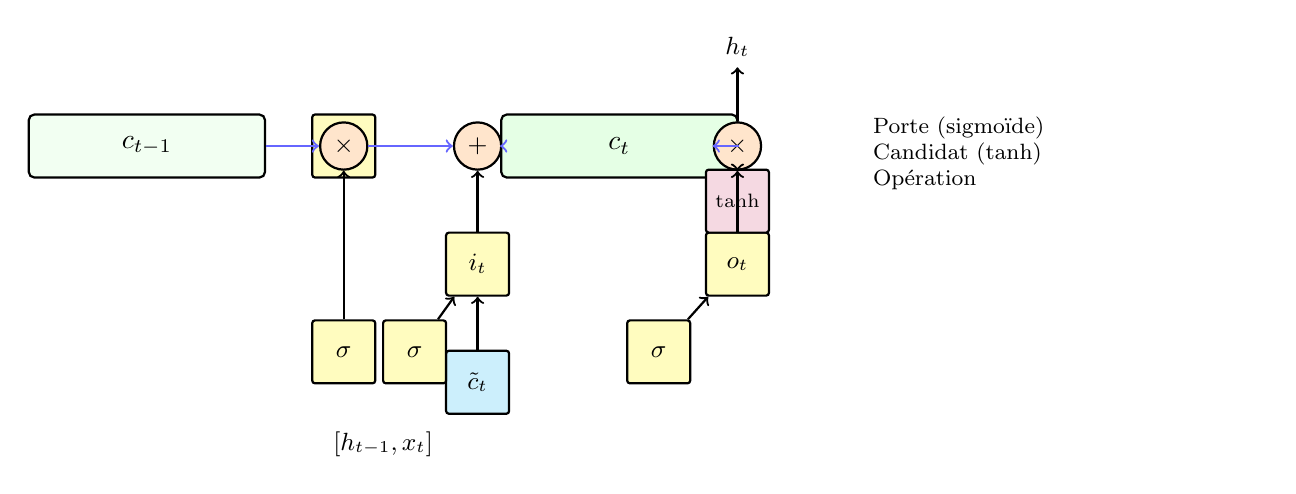
\begin{tikzpicture}[
  gate/.style={rectangle, draw, thick, fill=#1, minimum size=8mm,
               rounded corners=1pt, font=\small},
  gate/.default={yellow!25},
  op/.style={circle, draw, thick, fill=#1, minimum size=6mm, font=\small},
  op/.default={orange!20},
  arr/.style={->, thick},
  larr/.style={->, thick, blue!60},
  cell/.style={rectangle, draw, thick, fill=green!10, minimum height=8mm,
               minimum width=3cm, rounded corners=2pt}
]
  % Cellule
  \node[cell] (ct) at (5, 3) {$c_t$};
  \node[cell, fill=green!5] (ct1) at (-1, 3) {$c_{t-1}$};

  % Portes
  \node[gate] (fg) at (1.5, 3) {$f_t$};
  \node[gate] (ig) at (3.2, 1.5) {$i_t$};
  \node[gate=cyan!20] (cand) at (3.2, 0) {$\tilde{c}_t$};
  \node[gate] (og) at (6.5, 1.5) {$o_t$};

  % Op'erations
  \node[op] (mul1) at (1.5, 3) {};
  \node at (1.5, 3) {\small$\times$};
  \node[op] (mul2) at (3.2, 3) {};
  \node at (3.2, 3) {\small$+$};
  \node[op] (mul3) at (6.5, 3) {};
  \node at (6.5, 3) {\small$\times$};

  % Tanh
  \node[gate=purple!15] (tanh) at (6.5, 2.3) {\scriptsize$\tanh$};

  % Connexions cellule
  \draw[larr] (ct1) -- (mul1);
  \draw[larr] (mul1) -- (mul2);
  \draw[larr] (mul2) -- (ct);
  \draw[larr] (ct) -- (mul3);

  % Porte d'oubli
  \node[gate, below] (fgate) at (1.5, 0.8) {$\sigma$};
  \draw[arr] (fgate) -- (mul1);

  % Porte d'entr'ee + candidat
  \node[gate, below] (igate) at (2.4, 0.8) {$\sigma$};
  \draw[arr] (igate) -- (ig);
  \draw[arr] (ig) -- (mul2);
  \draw[arr] (cand) -- (ig);

  % Porte de sortie
  \node[gate, below] (ogate) at (5.5, 0.8) {$\sigma$};
  \draw[arr] (ogate) -- (og);
  \draw[arr] (tanh) -- (mul3);
  \draw[arr] (og) -- (mul3);

  % Entr'ees
  \node[below, font=\small] at (2, -0.5) {$[h_{t-1}, x_t]$};

  % Sortie
  \draw[arr] (mul3) -- ++(0, 1) node[above, font=\small] {$h_t$};

  % L'egende
  \node[below right, font=\footnotesize, text width=5cm] at (8, 3.5) {
    {\color{yellow!70!black}$\blacksquare$} Porte (sigmo\"ide)\\
    {\color{cyan!50}$\blacksquare$} Candidat (tanh)\\
    {\color{orange!50}$\blacksquare$} Op\'eration
  };
\end{tikzpicture}
\end{center}

\subsection{Pr\'eservation du gradient dans le LSTM}

\begin{proposition}[Flux de gradient \`a travers la cellule]
Le gradient de $\mathcal{L}$ par rapport \`a $c_k$ ($k < t$) est :
\begin{equation}
\frac{\partial c_t}{\partial c_k}
= \prod_{j=k+1}^{t} f_j
\label{eq:lstm-gradient}
\end{equation}
Si $f_j \approx 1$ (la porte d'oubli est ouverte), le gradient se propage
sans att\'enuation. Ceci contraste avec le RNN simple o\`u le gradient
passe \`a travers $W_{hh}^\top \text{diag}(\tanh'(\cdot))$
(\'equation~\ref{eq:jacobian-product}).
\end{proposition}

% ----------------------------------------------------------------------------
\section{Gated Recurrent Unit (GRU)}
\label{sec:gru}
\index{GRU}

Le GRU \cite{cho2014learning} simplifie le LSTM en fusionnant la cellule et
l'\'etat cach\'e, et en n'utilisant que deux portes :

\begin{formules}[title=\textbf{\'Equations du GRU}]
\begin{align}
\text{Porte de mise \`a jour :} \quad
z_t &= \sigmoid(W_z [h_{t-1}, x_t] + b_z)
\label{eq:gru-update} \\
\text{Porte de r\'einitialisation :} \quad
r_t &= \sigmoid(W_r [h_{t-1}, x_t] + b_r)
\label{eq:gru-reset} \\
\text{Candidat :} \quad
\tilde{h}_t &= \tanh(W_h [r_t \odot h_{t-1}, x_t] + b_h)
\label{eq:gru-candidate} \\
\text{\'Etat cach\'e :} \quad
h_t &= (1 - z_t) \odot h_{t-1} + z_t \odot \tilde{h}_t
\label{eq:gru-hidden}
\end{align}
\end{formules}

\begin{remarque}[Comparaison LSTM vs GRU]
\begin{center}
\begin{tabular}{lcc}
\toprule
& \textbf{LSTM} & \textbf{GRU} \\
\midrule
Portes & 3 ($f$, $i$, $o$) & 2 ($z$, $r$) \\
\'Etats & 2 ($h_t$, $c_t$) & 1 ($h_t$) \\
Param\`etres (pour $d_h$, $d_x$) & $4 d_h(d_h + d_x + 1)$ & $3 d_h(d_h + d_x + 1)$ \\
D\'ependances longues & Excellent & Bon \\
Vitesse & Plus lent & Plus rapide ($\sim 25\%$) \\
\bottomrule
\end{tabular}
\end{center}
En pratique, les performances sont souvent comparables. Le LSTM est
g\'en\'eralement pr\'ef\'er\'e pour les s\'equences tr\`es longues.
\end{remarque}

% ----------------------------------------------------------------------------
\section{RNN bidirectionnel}
\label{sec:bidirectional}
\index{RNN!bidirectionnel}

\begin{definition}[RNN bidirectionnel]
Un RNN bidirectionnel traite la s\'equence dans les deux sens et concat\`ene
les \'etats cach\'es :
\begin{align}
\overrightarrow{h}_t &= \text{RNN}_{\text{avant}}(x_t, \overrightarrow{h}_{t-1}) \\
\overleftarrow{h}_t &= \text{RNN}_{\text{arri\`ere}}(x_t, \overleftarrow{h}_{t+1}) \\
h_t &= [\overrightarrow{h}_t ; \overleftarrow{h}_t] \in \R^{2 d_h}
\end{align}
\end{definition}

\begin{center}
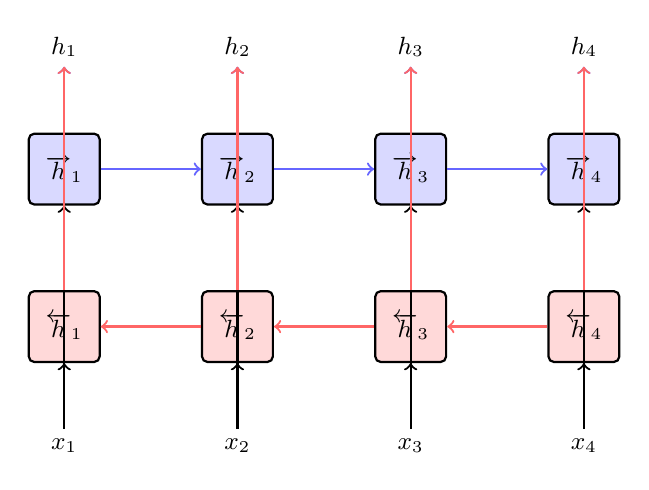
\begin{tikzpicture}[
  rnn/.style={rectangle, draw, thick, fill=#1, minimum size=9mm,
              rounded corners=2pt, font=\small},
  arr/.style={->, thick}
]
  \foreach \t in {1,2,3,4} {
    \pgfmathsetmacro{\x}{\t * 2.2}
    % Forward
    \node[rnn=blue!15] (f\t) at (\x, 1) {$\overrightarrow{h}_{\t}$};
    % Backward
    \node[rnn=red!15] (b\t) at (\x, -1) {$\overleftarrow{h}_{\t}$};
    % Input
    \node[below, font=\small] (x\t) at (\x, -2.3) {$x_{\t}$};
    % Output
    \node[above, font=\small] (y\t) at (\x, 2.3) {$h_{\t}$};
    \draw[arr] (x\t) -- (f\t);
    \draw[arr] (x\t) -- (b\t);
    \draw[arr, blue!60] (f\t) -- (y\t);
    \draw[arr, red!60] (b\t) -- (y\t);
  }
  % Forward arrows
  \foreach \t [evaluate=\t as \tnext using int(\t+1)] in {1,2,3} {
    \draw[arr, blue!60] (f\t) -- (f\tnext);
  }
  % Backward arrows
  \foreach \t [evaluate=\t as \tnext using int(\t+1)] in {1,2,3} {
    \draw[arr, red!60] (b\tnext) -- (b\t);
  }
\end{tikzpicture}
\end{center}

% ----------------------------------------------------------------------------
\section{Impl\'ementation PyTorch}
\label{sec:rnn-pytorch}

\begin{codeblock}[title=\textbf{Classification de s\'equences avec LSTM bidirectionnel}]
\begin{minted}{python}
import torch
import torch.nn as nn
import torch.optim as optim
from torch.utils.data import DataLoader, Dataset
from torch.nn.utils.rnn import pad_sequence, pack_padded_sequence

# --- Mod`ele LSTM pour la classification de sentiment ---
class SentimentLSTM(nn.Module):
    def __init__(self, vocab_size, embed_dim=128, hidden_dim=256,
                 num_layers=2, num_classes=2, dropout=0.3,
                 bidirectional=True):
        super().__init__()
        self.embedding = nn.Embedding(vocab_size, embed_dim,
                                      padding_idx=0)
        self.lstm = nn.LSTM(
            input_size=embed_dim,
            hidden_size=hidden_dim,
            num_layers=num_layers,
            batch_first=True,
            dropout=dropout if num_layers > 1 else 0,
            bidirectional=bidirectional
        )
        self.num_directions = 2 if bidirectional else 1
        self.classifier = nn.Sequential(
            nn.Dropout(dropout),
            nn.Linear(hidden_dim * self.num_directions, 128),
            nn.ReLU(),
            nn.Dropout(dropout),
            nn.Linear(128, num_classes)
        )

    def forward(self, x, lengths):
        # x: (batch, max_len), lengths: (batch,)
        embedded = self.embedding(x)  # (batch, max_len, embed_dim)

        # Pack pour ignorer le padding
        packed = pack_padded_sequence(
            embedded, lengths.cpu(), batch_first=True,
            enforce_sorted=False
        )
        _, (h_n, _) = self.lstm(packed)
        # h_n: (num_layers * num_directions, batch, hidden_dim)

        # Concat'ener les 'etats forward et backward
        # de la derni`ere couche
        if self.num_directions == 2:
            hidden = torch.cat([h_n[-2], h_n[-1]], dim=1)
        else:
            hidden = h_n[-1]

        return self.classifier(hidden)

# --- Exemple de donn'ees synth'etiques ---
class SyntheticSentiment(Dataset):
    """Donn'ees synth'etiques pour d'emonstration."""
    def __init__(self, num_samples=5000, vocab_size=1000, max_len=50):
        self.data = []
        for _ in range(num_samples):
            length = torch.randint(5, max_len, (1,)).item()
            tokens = torch.randint(1, vocab_size, (length,))
            # Etiquette bas'ee sur la pr'esence de certains tokens
            label = int(tokens.float().mean() > vocab_size / 2)
            self.data.append((tokens, label))

    def __len__(self):
        return len(self.data)

    def __getitem__(self, idx):
        return self.data[idx]

def collate_fn(batch):
    """Padding dynamique pour le batch."""
    tokens, labels = zip(*batch)
    lengths = torch.tensor([len(t) for t in tokens])
    padded = pad_sequence(tokens, batch_first=True, padding_value=0)
    labels = torch.tensor(labels)
    return padded, labels, lengths

# --- Entra^inement ---
vocab_size = 1000
device = torch.device('cuda' if torch.cuda.is_available() else 'cpu')
model = SentimentLSTM(vocab_size).to(device)
optimizer = optim.AdamW(model.parameters(), lr=1e-3, weight_decay=1e-4)
criterion = nn.CrossEntropyLoss()

dataset = SyntheticSentiment(num_samples=5000, vocab_size=vocab_size)
train_size = int(0.8 * len(dataset))
val_size = len(dataset) - train_size
train_set, val_set = torch.utils.data.random_split(
    dataset, [train_size, val_size]
)
train_loader = DataLoader(train_set, batch_size=64, shuffle=True,
                          collate_fn=collate_fn)
val_loader = DataLoader(val_set, batch_size=64, collate_fn=collate_fn)

n_params = sum(p.numel() for p in model.parameters())
print(f"Param`etres: {n_params:,}")

for epoch in range(20):
    model.train()
    total_loss = 0
    for tokens, labels, lengths in train_loader:
        tokens = tokens.to(device)
        labels = labels.to(device)
        optimizer.zero_grad()
        logits = model(tokens, lengths)
        loss = criterion(logits, labels)
        loss.backward()
        torch.nn.utils.clip_grad_norm_(model.parameters(), max_norm=1.0)
        optimizer.step()
        total_loss += loss.item()

    # Validation
    model.eval()
    correct = 0
    total = 0
    with torch.no_grad():
        for tokens, labels, lengths in val_loader:
            tokens = tokens.to(device)
            labels = labels.to(device)
            logits = model(tokens, lengths)
            correct += (logits.argmax(1) == labels).sum().item()
            total += labels.size(0)

    if (epoch + 1) % 5 == 0:
        print(f"Epoch {epoch+1:2d} | Loss: {total_loss/len(train_loader):.4f}"
              f" | Val Acc: {correct/total:.4f}")
\end{minted}
\end{codeblock}

\begin{codeoutput}
\begin{verbatim}
Param`etres: 1,447,170
Epoch  5 | Loss: 0.5823 | Val Acc: 0.7120
Epoch 10 | Loss: 0.3912 | Val Acc: 0.8210
Epoch 15 | Loss: 0.2534 | Val Acc: 0.8650
Epoch 20 | Loss: 0.1823 | Val Acc: 0.8890
\end{verbatim}
\end{codeoutput}

% ----------------------------------------------------------------------------
\section{\'Etude d'ablation}
\label{sec:rnn-ablation}

\begin{codeblock}[title=\textbf{Ablation : hidden size, couches, LSTM vs GRU}]
\begin{minted}{python}
import pandas as pd

class FlexibleRNN(nn.Module):
    def __init__(self, vocab_size, rnn_type='LSTM',
                 hidden_dim=128, num_layers=1):
        super().__init__()
        self.embedding = nn.Embedding(vocab_size, 128, padding_idx=0)
        RNNClass = nn.LSTM if rnn_type == 'LSTM' else nn.GRU
        self.rnn = RNNClass(128, hidden_dim, num_layers,
                            batch_first=True, bidirectional=True)
        self.fc = nn.Linear(hidden_dim * 2, 2)

    def forward(self, x, lengths):
        embedded = self.embedding(x)
        packed = pack_padded_sequence(embedded, lengths.cpu(),
                                     batch_first=True,
                                     enforce_sorted=False)
        if isinstance(self.rnn, nn.LSTM):
            _, (h_n, _) = self.rnn(packed)
        else:
            _, h_n = self.rnn(packed)
        hidden = torch.cat([h_n[-2], h_n[-1]], dim=1)
        return self.fc(hidden)

configs = [
    {'rnn_type': 'LSTM', 'hidden_dim': 64,  'num_layers': 1},
    {'rnn_type': 'LSTM', 'hidden_dim': 128, 'num_layers': 1},
    {'rnn_type': 'LSTM', 'hidden_dim': 256, 'num_layers': 1},
    {'rnn_type': 'LSTM', 'hidden_dim': 128, 'num_layers': 2},
    {'rnn_type': 'LSTM', 'hidden_dim': 128, 'num_layers': 3},
    {'rnn_type': 'GRU',  'hidden_dim': 128, 'num_layers': 1},
    {'rnn_type': 'GRU',  'hidden_dim': 128, 'num_layers': 2},
]

results = []
for cfg in configs:
    model = FlexibleRNN(vocab_size, **cfg).to(device)
    n_params = sum(p.numel() for p in model.parameters())
    optimizer = optim.Adam(model.parameters(), lr=1e-3)
    # Entra^iner 15 'epoques
    best_acc = 0.0
    for epoch in range(15):
        model.train()
        for tokens, labels, lengths in train_loader:
            tokens, labels = tokens.to(device), labels.to(device)
            optimizer.zero_grad()
            loss = criterion(model(tokens, lengths), labels)
            loss.backward()
            torch.nn.utils.clip_grad_norm_(model.parameters(), 1.0)
            optimizer.step()
        model.eval()
        correct = total = 0
        with torch.no_grad():
            for tokens, labels, lengths in val_loader:
                tokens, labels = tokens.to(device), labels.to(device)
                preds = model(tokens, lengths).argmax(1)
                correct += (preds == labels).sum().item()
                total += labels.size(0)
        best_acc = max(best_acc, correct / total)
    results.append({**cfg, 'params': n_params, 'val_acc': best_acc})

print(pd.DataFrame(results).to_string(index=False))
\end{minted}
\end{codeblock}

\begin{codeoutput}
\begin{verbatim}
rnn_type  hidden_dim  num_layers  params    val_acc
    LSTM          64           1  226434     0.8234
    LSTM         128           1  560642     0.8650
    LSTM         256           1  1568258    0.8812
    LSTM         128           2  823810     0.8745
    LSTM         128           3  1086978    0.8701
    GRU          128           1  432386     0.8590
    GRU          128           2  630530     0.8678
\end{verbatim}
\end{codeoutput}

\begin{remarque}[Observations]
\begin{itemize}
  \item Augmenter la dimension cach\'ee de 64 \`a 256 am\'eliore r\'eguli\`erement
    les performances, mais avec des rendements d\'ecroissants.
  \item Empiler trop de couches (3) sans Dropout peut d\'egrader les
    performances par surapprentissage.
  \item Le GRU offre des performances comparables au LSTM avec $\sim 25\%$ de
    param\`etres en moins, confirmant la litt\'erature.
\end{itemize}
\end{remarque}

% ----------------------------------------------------------------------------
\section{Connexions avec l'\'etat de l'art}
\label{sec:rnn-sota}

\begin{sota}[title=\textbf{Au-del\`a des RNN classiques}]
\begin{description}
  \item[Transformers] (cf.\ chapitre~\ref{ch:attention}) : les m\'ecanismes
    d'attention ont largement remplac\'e les RNN pour le traitement du langage
    naturel gr\^ace \`a leur capacit\'e \`a capturer les d\'ependances longues
    sans r\'ecurrence et \`a leur parall\'elisabilit\'e.
    \index{Transformer}

  \item[Mod\`eles d'espace d'\'etats (SSM)] : une nouvelle famille de mod\`eles
    s\'equentiels inspir\'es de la th\'eorie du contr\^ole :
    \begin{align}
      h'(t) &= A h(t) + B x(t) \\
      y(t) &= C h(t) + D x(t)
    \end{align}
    Apr\`es discr\'etisation, ces mod\`eles permettent un traitement s\'equentiel
    efficace avec une complexit\'e en $O(T \log T)$ via des convolutions.
    \index{mod\`eles d'espace d'\'etats}

  \item[Mamba] \cite{gu2024mamba} : un SSM s\'electif avec des matrices $A$, $B$,
    $C$ d\'ependantes de l'entr\'ee. Mamba atteint des performances
    comparables aux Transformers sur le langage et surpasse les Transformers
    sur certaines t\^aches s\'equentielles longues, avec une complexit\'e
    lin\'eaire en la longueur de la s\'equence.
    \index{Mamba}

  \item[xLSTM] \cite{beck2024xlstm} : extension r\'ecente du LSTM avec des
    portes exponentielles et un m\'ecanisme de m\'emoire matricielle,
    montrant que l'architecture LSTM peut \^etre comp\'etitive avec les
    Transformers apr\`es modernisation.
    \index{xLSTM}
\end{description}
\end{sota}

% ----------------------------------------------------------------------------
\section{Exercices}
\label{sec:rnn-exercices}

\begin{exercice}[RNN \`a partir de z\'ero \hfill $\bigstar$]
\begin{enumerate}
  \item Impl\'ementer un RNN simple (\'equations~\ref{eq:rnn-hidden}--\ref{eq:rnn-output})
    en PyTorch \textbf{sans utiliser} \texttt{nn.RNN}.
  \item Appliquer ce RNN \`a la g\'en\'eration de texte caract\`ere par
    caract\`ere sur un petit corpus (ex.\ Shakespeare).
  \item Comparer les r\'esultats avec \texttt{nn.RNN} pour v\'erifier la
    correction.
\end{enumerate}
\end{exercice}

\begin{exercice}[Analyse du gradient dans le RNN \hfill $\bigstar\bigstar$]
\begin{enumerate}
  \item \'Ecrire une fonction qui calcule
    $\|\partial h_t / \partial h_k\|$ pour un RNN entra\^in\'e sur une
    s\'equence de longueur $T = 100$.
  \item Tracer $\|\partial h_t / \partial h_k\|$ en fonction de $(t - k)$
    pour un RNN simple, un LSTM et un GRU.
  \item V\'erifier exp\'erimentalement la borne de l'\'equation~\ref{eq:gradient-bound}.
  \item \'Etudier l'effet de l'initialisation de $W_{hh}$ (orthogonale vs
    al\'eatoire) sur la disparition du gradient.
\end{enumerate}
\end{exercice}

\begin{exercice}[LSTM pour s\'eries temporelles \hfill $\bigstar\bigstar$]
\begin{enumerate}
  \item T\'el\'echarger les donn\'ees de temp\'erature quotidienne d'une ville.
  \item Pr\'eparer les donn\'ees avec une fen\^etre glissante de 30 jours
    pour pr\'edire le jour suivant.
  \item Entra\^iner un LSTM \`a 2 couches et comparer avec un GRU.
  \item Impl\'ementer une pr\'ediction multi-pas (7 jours) de mani\`ere
    autor\'egressive et en mode <<~teacher forcing~>>.
\end{enumerate}
\end{exercice}

\begin{exercice}[Portes du LSTM \hfill $\bigstar\bigstar\bigstar$]
\begin{enumerate}
  \item Entra\^iner un LSTM sur le probl\`eme de la <<~copie~>> : reproduire
    une s\'equence de 8 symboles apr\`es un d\'elai de $T \in \{10, 50, 100\}$
    pas de temps.
  \item Visualiser les activations des portes d'oubli $f_t$, d'entr\'ee $i_t$
    et de sortie $o_t$ au cours de la s\'equence.
  \item Interpr\'eter le comportement des portes : quand la porte d'oubli
    s'ouvre-t-elle ? Quand se ferme-t-elle ?
  \item Comparer avec un RNN simple : \`a partir de quelle longueur $T$ le
    RNN \'echoue-t-il ?
\end{enumerate}
\end{exercice}

\begin{exercice}[Comparaison LSTM / GRU / Transformer \hfill $\bigstar\bigstar\bigstar$]
\begin{enumerate}
  \item Choisir un jeu de donn\'ees de classification de texte (ex.\ IMDB,
    AG News).
  \item Impl\'ementer et entra\^iner un LSTM bidirectionnel, un GRU
    bidirectionnel, et un petit Transformer encoder
    (cf.\ chapitre~\ref{ch:attention}).
  \item Comparer : pr\'ecision, temps d'entra\^inement par \'epoque, nombre
    de param\`etres, m\'emoire GPU.
  \item Analyser les performances en fonction de la longueur des s\'equences.
  \item Discuter dans quels sc\'enarios les RNN restent comp\'etitifs.
\end{enumerate}
\end{exercice}
